\label{chapter:improvements}

In this chapter we look at two improvements to the binary XPFC theory. Both of
these improvements are novel contributions to the field and significantly
extend the scope of the XPFC framework. The improvements, as previously eluded
to, are to first, extend the the free energy to mixing in the XPFC model to one
with an enthalpy of mixing and to second, generalize the phenomenological form
used to model correlation functions.

%%%%%%%%%%%%%%%%%%%%%%%%%%%%%%%%%%%
\section{Regular Mixing Model} %
%%%%%%%%%%%%%%%%%%%%%%%%%%%%%%%%%%%

Extending the free energy of mixing beyond ideal mixing is achieved by removing
the assumption made by Greenwood \textit{et al.} in deriving the binary XPFC
model that the concentration-concentration correlation function has no $k=0$ mode.
This is the same approach taken in the original model, though we keep the ideal
mixing term unexpanded as in the XPFC model. The correlation function is expanded
as,
%
\begin{equation}
    C_{cc}(r, r^\prime) = \d(r - r^\prime)
        \l(\omega\epsilon + W_c\nabla^2 + \cdots\r).
\end{equation}
%
This form results in a free energy functional of the form,
%
\begin{align}
    \f{\beta\Delta\F[n, c]}{\rho_0} &= \integrate{r} \l\lbrace
        \f{1}{2} n(r) \l(1 - C_{nn}(r, r^\prime)\r) \ast n(r^\prime)
        - \eta \f{n^3}{6} + \chi \f{n^4}{12} \r\rbrace \\
        &+ \integrate{r}\l\lbrace
            \f{1}{2}\l\vert \nabla c(r) \r\vert^2 + \omega f_{mix}(r)
            \r\rbrace. \nonumber
\end{align}
%
Where the local free energy density of mixing, $f_{mix}$ is now,
%
\begin{equation}
    f_{mix}(r) = \l(n(r) + 1\r)\l(
            c(r)\ln\l(\f{c(r)}{c_0}\r)
          + (1-c(r))\ln\l(\f{1-c(r)}{1-c_0}\r) \r)
          + \f{1}{2} \epsilon (c - c_0)^2.
\end{equation}
%
For simplicity the temperature dependence of the parameter $\epsilon$ is taken
to be linear about a spinodal temperature $T_c$,
%
\begin{equation}
    \epsilon(T) = -4 + \epsilon_0(T - T_c).
\end{equation}
%
The resulting model has a free energy of mixing that is equivalent to the
regular solution model and, as such, it makes a clear connection to a well
used model else where in material science. The regular solution model
also supplies the essential physics of a non-negligible enthalpy of mixing.

%%%%%%%%%%%%%%%%%%%%%%%%%%%%%%%%%%%%%%%%%%%%%%
\section{General Correlation Function Model} %
%%%%%%%%%%%%%%%%%%%%%%%%%%%%%%%%%%%%%%%%%%%%%%

To establish a general phenomenology for modelling density-density 
correlation functions note that the density-density correlation function
as the form of a linear combination of interpolating functions in
concentration, $\zeta(c)$, multiplied by bare correlation functions $C(r,
r^\prime)$,
%
\begin{equation}
    C_{nn}(r, r^\prime; c) = \sum_i \zeta_i(c) C_i(r, r^\prime)
\end{equation}
%
In the exact theory, for example, we have,
%
\begin{gather}
    \zeta_{AA}(c) = \rho_0 (1 - c^2), \\
    \zeta_{AB}(c) = \rho_0 c (1 - c ), \\
    \zeta_{BB}(c) = \rho_0 c^2.
\end{gather}
%
Each interpolating function, $\zeta_i(c)$, defines a domain of validity for its
associated correlation function $C_i(r, r^\prime)$. This suggests that we might
model any density-density correlation function using this general structure:
the set of correlation function $C_i(r, r^\prime)$ enumerate the various
structures (correlations) that may manifest themselves and the associated
interpolation functions $\zeta_i(c)$ define the concentrations over which these
correlations are valid.

As a simple example if we wanted to construct a simple model of the
silver-cupper eutectic alloy system, we might start with some model correlation
function for pure silver, $C_\alpha(r, r^\prime)$, and for pure copper,
$C_\beta(r, r^\prime)$. These two structures, the silver rich $\alpha$ phase
and the copper rich $\beta$ phase, are the only two relevent crystalline
structures in the system so to build the full density-density correlation
function we just need to choose interpolating functions for each. Following
Greenwood \textit{et al} for example, we might choose,
%
\begin{gather}
    \zeta_\alpha(c) = 1 - 3c^2 + 2c^3, \\
    \zeta_\beta(c) = 1 - 3 (1 - c)^2 + 2(1 - c)^3.
\end{gather}
%
To model the $\alpha$ and $\beta$ correlation functions we use the original
XPFC formalism for modelling bare correlation functions. The $\alpha$ and 
$\beta$ phase are both FCC \cite{SUBRAMANIAN93} so we can use an FCC model for the correlation 
function as in \cite{GREENWOOD10}.

%%%%%%%%%%%%%%%%%%%%%%%%%%%%%%%%%%
\section{Equilibrium Properties} %
%%%%%%%%%%%%%%%%%%%%%%%%%%%%%%%%%%

These two changes to the XPFC formalism extend the possible systems we can 
study. In this section we'll explore the equilibrium properties of the
improved XPFC free energy functional specialized for three different material
phase diagrams: eutectic, syntectic and monotectic.

%%%%%%%%%%%%%%%%%%%%%%%%%%%%%%%%%%%%%
\subsection{Eutectic Phase Diagram} %
%%%%%%%%%%%%%%%%%%%%%%%%%%%%%%%%%%%%%

While previous PFC models have shown that elastic energy is a sufficient
driving force for eutectic solidification our simplified regular model allows
for the examination of the role enthalpy of mixing can play in eutectic solids.
For instance, Murdoch and Schuh noted that in nanocrystalline binary alloys,
while a positive enthaply of segregation can stabilize against grain growth via
solute segregation at the grain boundary, if the enthaply of mixing becomes too
large this effect can be negated by second phase formation or even macroscopic
phase seperation\cite{MURDOCH13}. 

To specialize our simplified regular model to the case of the binary eutectic
we must choose an appropriate model for the correlation function. Choosing an
$\alpha$ phase around $c = 0$ and $\beta$ phase around $c = 1$, we can recover
the pair correlation function used in the binary XPFC with a
particular choice of window functions: 
%
\begin{align}
   \zeta_\alpha(c) &= 2c^3 - 3c^2 + 1 \\
   \zeta_\beta(c) &= \zeta_\alpha(1 - c).
\end{align}
%
Should we choose, for example, an $\alpha$ and $\beta$ phase with 2 dimensional
hexagonal lattices, differing only by lattice constants, we can produce a phase
diagram like that in Fig. \ref{eutectic}.  

\begin{figure}[h]
    \centering	
    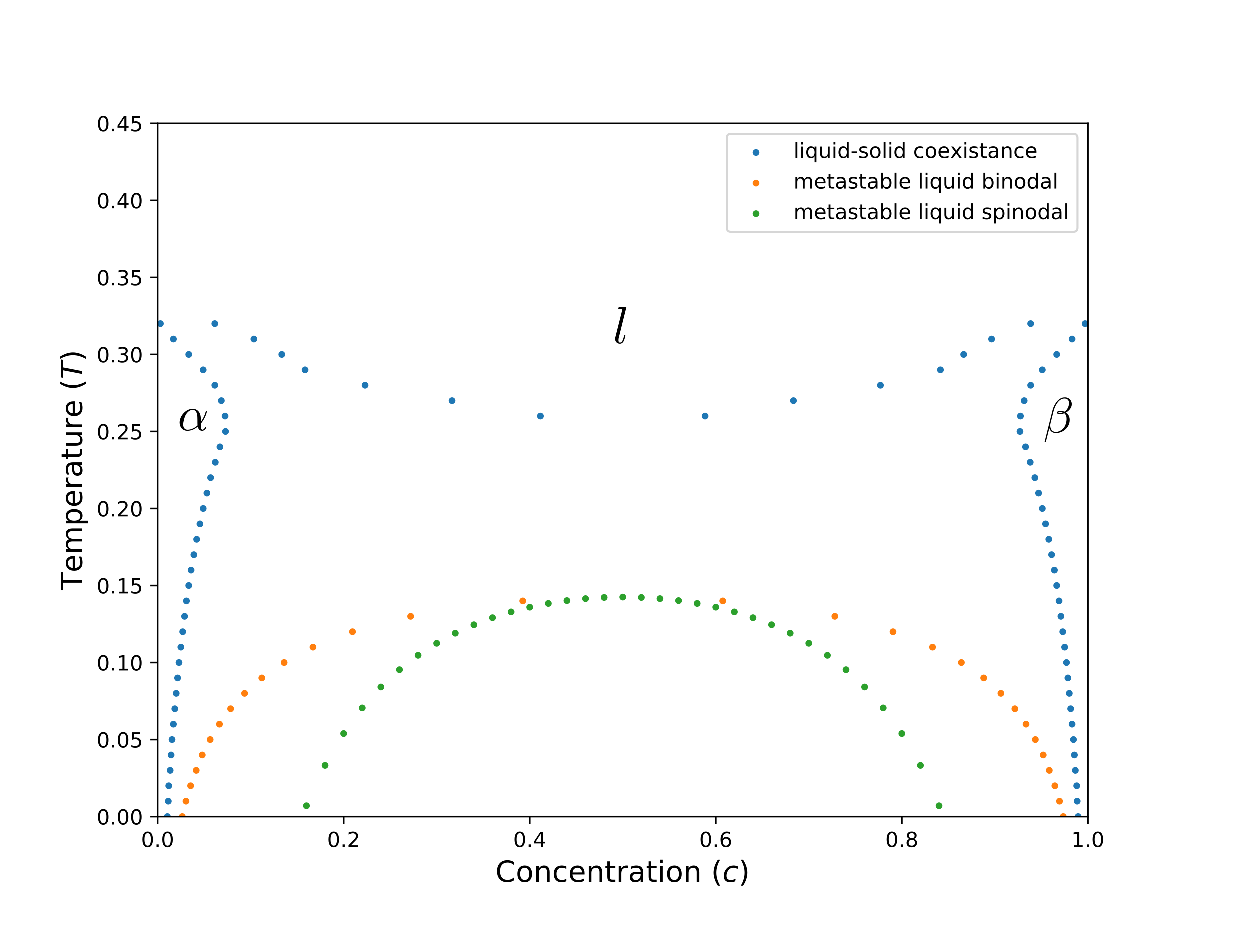
\includegraphics[scale=0.7]{eutectic}
    \caption[Eutectic Phase Diagram]{
        \label{eutectic} Eutectic phase diagram triangle $\alpha$ and $\beta$
        phases. The free energy parameter are $\eta = 2$, $\chi = 1$,
        $\omega=0.30$, $\epsilon_0 = 3$ and $T_c = 0.01$. The parameters of the
        structure functions are $\alpha_{10\alpha} = \alpha_{10\beta} = 0.8$,
        $k_{10\alpha} = 2\pi$, $k_{10\beta} = 4\pi/\sqrt{3}$ and $T_0 = 1$
    }
\end{figure}

%%%%%%%%%%%%%%%%%%%%%%%%%%%%%%%%%%%%%%
\subsection{Syntectic Phase Diagram} %
%%%%%%%%%%%%%%%%%%%%%%%%%%%%%%%%%%%%%%

Our regular model also allows for the study of a variety of invariant binary
reactions that, to date, have not been studied using phase field crystal
models. One such reaction is the syntectic reaction. 

The syntectic reaction, $l_1 + l_2 \rightarrow \alpha $, consists of
solidification at the interface of two liquids. We can achieve this with our
model by setting the spinodal temperature, $T_c$, sufficiently high and
producing a density-density correlation function that is peaked at a
concentration below the spinodal. This can be done by choosing a window
function that is centered about an intermediate concentration, $c_\alpha$ of
the solid phase, $\alpha$. 
%
\begin{equation}
  \chi(c) = e^{- \f{(c - c_\alpha)^2}{2 \alpha_c}}
\end{equation}
%
The resulting correlation function for a hexagonal lattice in two dimensions,
for example, would be,
%
\begin{equation}
  \tilde{C}_{nn}(k; c) = 
    e^{-\f{(c - c_\alpha)^2}{2 \alpha_c}}
    e^{-\f{T}{T_0}} 
    e^{-\f{(k - k^\prime)^2}{2\alpha^2}}
\end{equation}
%
A phase diagram that produces a syntectic reaction with an appropriate choice
of parameters can be seen in Fig. \ref{syntectic}.

\begin{figure}
    \centering
	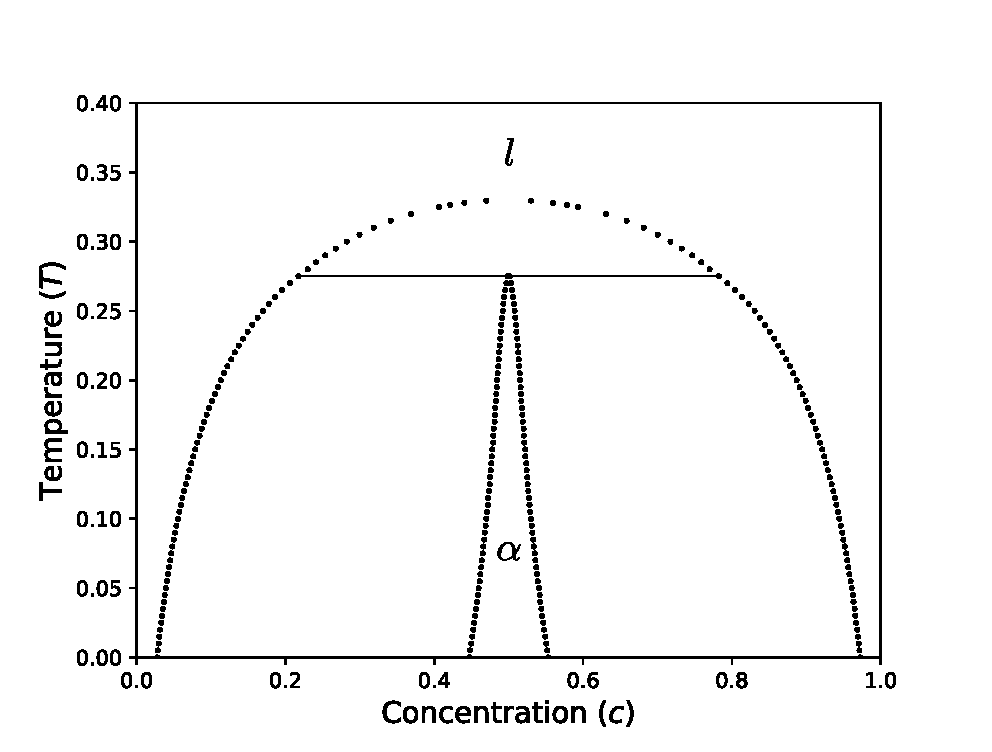
\includegraphics[scale=0.7]{syntectic.eps}
    \caption[Syntectic Phase Diagram]{
        \label{syntectic} Phase Diagram of Syntectic Alloy with a hexagonal
        $\alpha$ phase. The free energy parameters are $\eta=2$, $\chi=1$,
        $\omega=0.3$, $\epsilon_0 = 10$ and $T_c=0.35$. The parameters for the
        structure function are $\alpha_{10\alpha} = 0.8$, $k_{10\alpha} = 2\pi$
        and $T_0 = 1$
    }
\end{figure}

%%%%%%%%%%%%%%%%%%%%%%%%%%%%%%%%%%%%%%%
\subsection{Monotectic Phase Diagram} %
%%%%%%%%%%%%%%%%%%%%%%%%%%%%%%%%%%%%%%%

The monotectic reaction is another invariant binary reaction that has not
previously been studied using PFC models. The monotectic reaction, $l_1
\rightarrow \alpha + l_2$, consists of decomposing liquid into a solute poor
solid and solute rich liquid. To model a monotectic using our regular model we
hypothesize a solid phase at $c=0$ and set the spinondal temperature higher
than the solidification temperature. To achieve this we use a window function
peaked around $c = 0$,
%
\begin{equation}
    \chi_\alpha(c) = e^{-\f{c^2}{2\alpha_c^2}}.
\end{equation}
%
Again considering a simple hexagonal lattice for the $\alpha$ phase, we can
produce a phase diagram with a monotectic reaction with an appropriate choice
of parameters as in Fig. \ref{monotectic}.

\begin{figure}
    \centering
	\includegraphics[scale=0.7]{monotectic.eps}
    \caption[Monotectic Phase Diagram]{
        \label{monotectic} Phase Diagram of Monotectic Alloy with hexagonal
        $\alpha$ phase. The free energy parameters are $\eta = 2$, $\chi=1$,
        $\omega=0.3$, $\epsilon_0 = 10$, $T_c = 0.35$ and $c_0 = 0.75$. The
        parameters for the structure function are $\alpha_{10\alpha} = 0.8$,
        $k_{10\alpha} = 2\pi$ and $T_0 = 1$ and the parameter for the window
        function is $\alpha_c = 0.4$
    }
\end{figure}

As we can see, our improvements not only reveal new details in existing
systems, but also model new systems that haven't been explored with PFC methods
before. They provide a general framework to explore the landscape of possible
binary alloys with an emphasis that the liquid free energy is a crucial element
in this complete description.

